%% LyX 2.1.2 created this file.  For more info, see http://www.lyx.org/.
%% Do not edit unless you really know what you are doing.
\documentclass[english]{article}
\usepackage[T1]{fontenc}
\usepackage[latin9]{inputenc}
\usepackage{babel}
\usepackage{graphicx}
\usepackage{float}
\setlength{\parindent}{0pt}

\begin{document}

\title{Lab 5: Moving Object Imaging\\ -------------------------------- \\ \Large Sensors and Digitization}
\author{ \ Armine Vardazaryan, Songyou Peng \\ arminevardazaryan@gmail.com, psy920710@gmail.com}
\date{6th November 2015}

\maketitle

\section*{Introduction}

Line scan cameras are imaging devices that instead of the usual matrix-shaped
arrangement of pixels, have just a single row of them. The lines are
continuously fed to a computer that joins them to each other and makes
an image. This is most commonly done by connecting the camera output
to a frame grabber which resides in a PCI slot of an industrial computer.\\%{[}1{]}

A line scan camera reads the image data one line at a time. This means that it doesn't observe the image as a whole, but rather reviews it
precisely line by line. This seamless recording style allows for inspections of over-long objects or even endless webs of material. These characteristics make line-scan cameras perfect for a variety of applications: The most common uses are quality assurance and sorting procedures. Its applications include video surveillance systems, satellite imaging, inspection of surfaces for flaws. When used for inspection purposes, the camera is usually used along with special software for detecting defects in materials(semi-conductions, paper, plastic, leather, etc.).\\

Another common use is for postal sorting or reading out barcodes,
QR codes, lines of text and other codes.\\%{[}2{]}

In this lab work we explore some of the properties of this type of line scan a camera.

\section*{Equipment and the setup}
The equipment for this lab work consisted of a  DALSA S2-1X-02K40 line scan camera with a PENTAX YF5028A-02 lens,a DALSA XCELERA-CL LX1 frame grabber, an oscilloscope, a pulse generator,a PC and moving industrial parts.
The experiment consisted of two parts: first we controlled the camera through the PC and the frame grabber, then an external signal generator was used to control the camera.

\section*{Image acquisition with a linear camera}

The goal of this first part of the experiment was to capture images of the moving object while also adjusting settings of the line scan camera.
We tried experimenting with various parameters in CamExpert and observed the effect on the obtained image. \\

Figure \ref{fig:first} shows how the moving object looks like at that moment with the line rate 1000 Hz. Correspondingly, the frame rate is 2.0 f/s.\\

\begin{figure}[H]
	\centering
	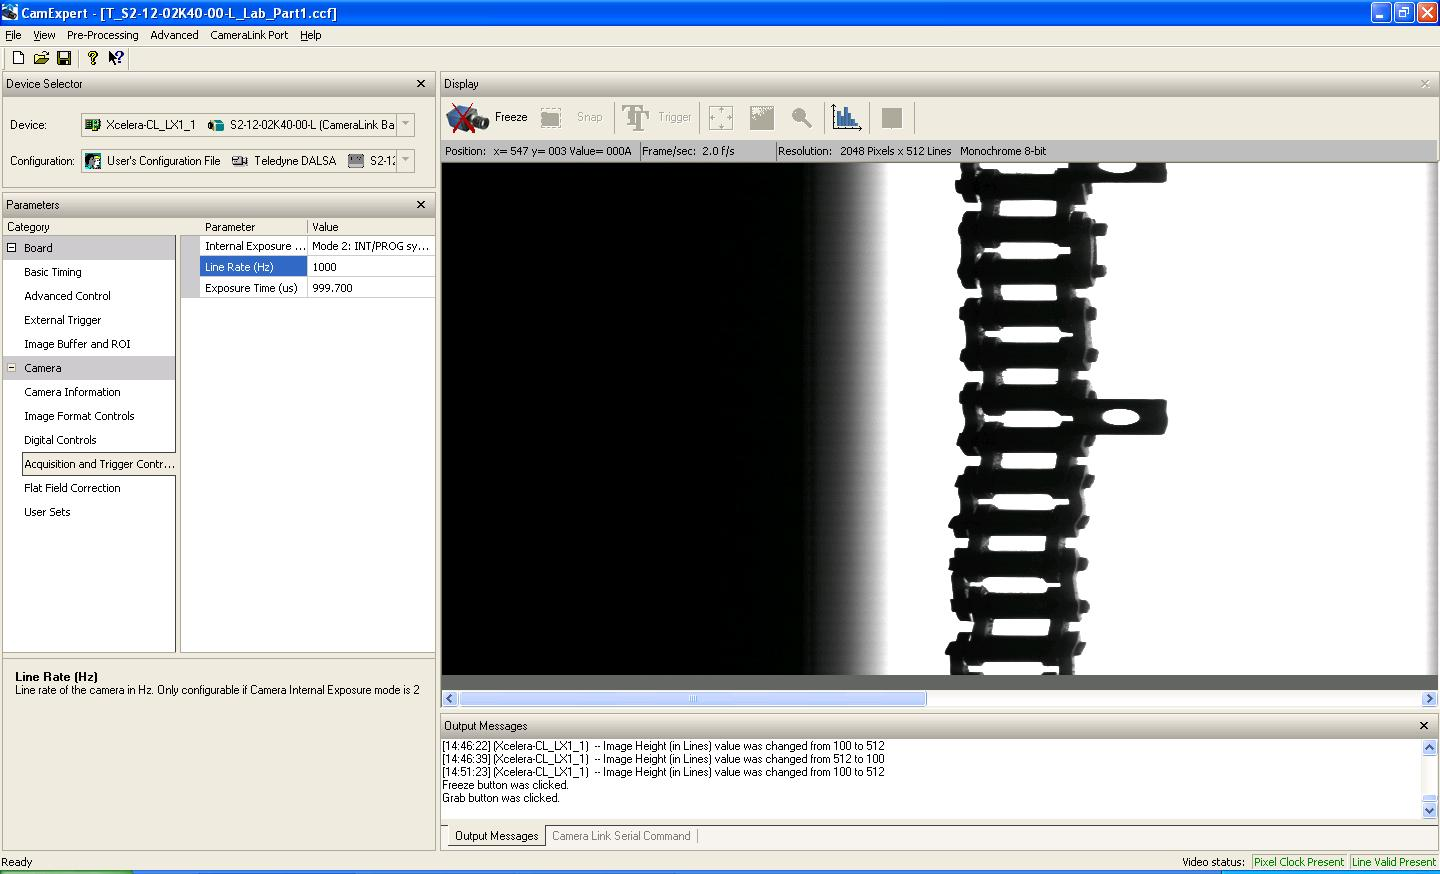
\includegraphics[width=\linewidth]{Pictures/1000.JPG}
	\caption{Line rate is 1000 Hz}
	\label{fig:first}
\end{figure}

When we increase the line rate to 10000 Hz, the moving object in the image we get becomes larger than that in 1000 Hz, which we are able to notice in Figure \ref{fig:second} . With the increase of line rate, frame rate also increases at the same time. Therefore, we can get more details of the same object part during a unit time and the object in the image is stretched as a result. And when the object is not moving, the image consists only of vertical lines or we can say that the same line is replicated throughout the image. We can conclude that this type of image contains not only spacial information but also information about the speed of the moving part.\\

\begin{figure}[H]
	\centering
	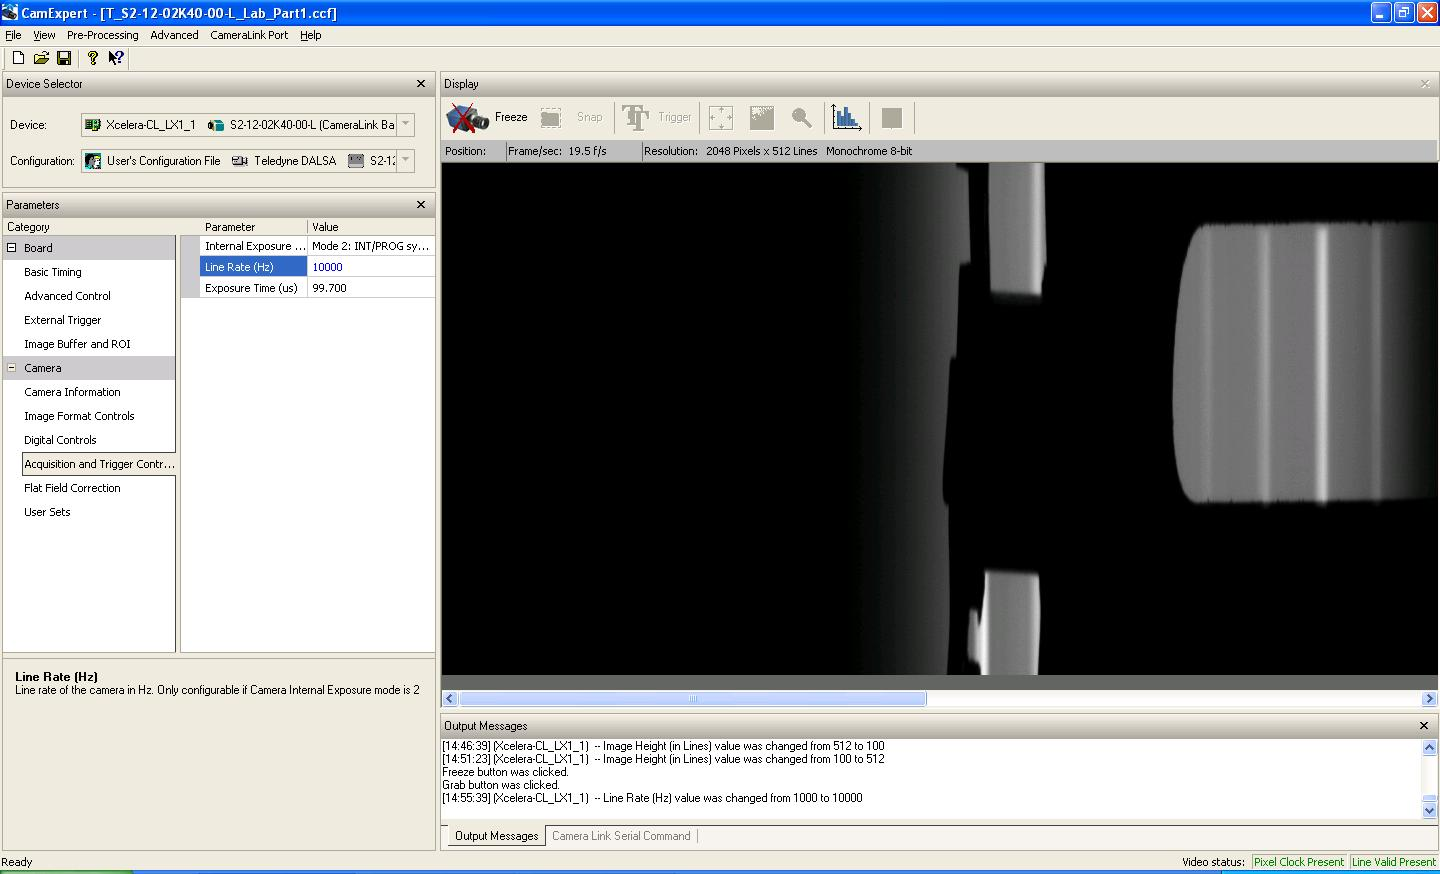
\includegraphics[width=\linewidth]{Pictures/10000.JPG}
	\caption{Line rate is 10000 Hz}
	\label{fig:second}
\end{figure}


We also try to change resolution, but it could not be done as the camera did not support any resolution other than its full value of 2048 pixels. However, the height of the image, could be adjusted. Because a smaller image requires less memory, the frame rate is affected by the image size as well. When the height is increased, the frame rate falls, and vice versa. This can be seen by comparing Figure \ref{fig:first} and Figure \ref{fig:third}: in both images the line rate is the same, the frame rate, however, is five times greater for the smaller image.

\begin{figure}[H]
	\centering
	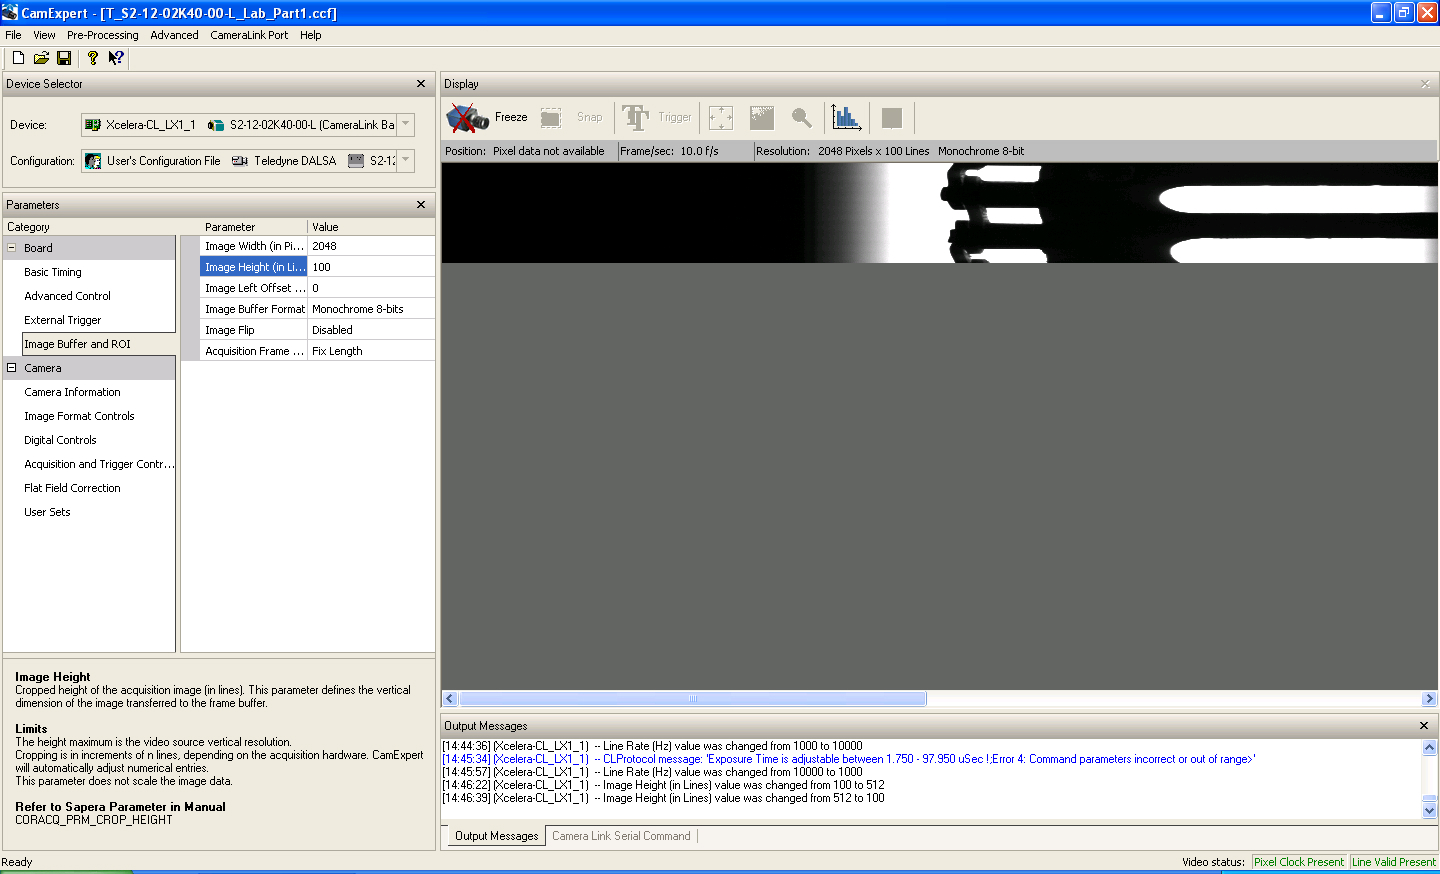
\includegraphics[width=\linewidth]{Pictures/third.jpg}
	\caption{Image height is changed from original 512 pixels to 100 pixels}
	\label{fig:third}
\end{figure}


\section*{Camera triggering by an external signal}

In this part of the experiment the camera was triggered by an external source: a signal generator. A rectangular signal of a set frequency was used to control the frame rate of the camera. Because the frame rate depends on the size of the available memory, and the line rate is limited by the frame rate, the image quality can also affected. Also, the externally set frame rate cannot be arbitrarily chosen, it must be less than or equal to the frame rate of the camera.\\
Figure \ref{fig:fourth} is an example of the camera working in this mode.\\

\begin{figure}[H]
	\centering
	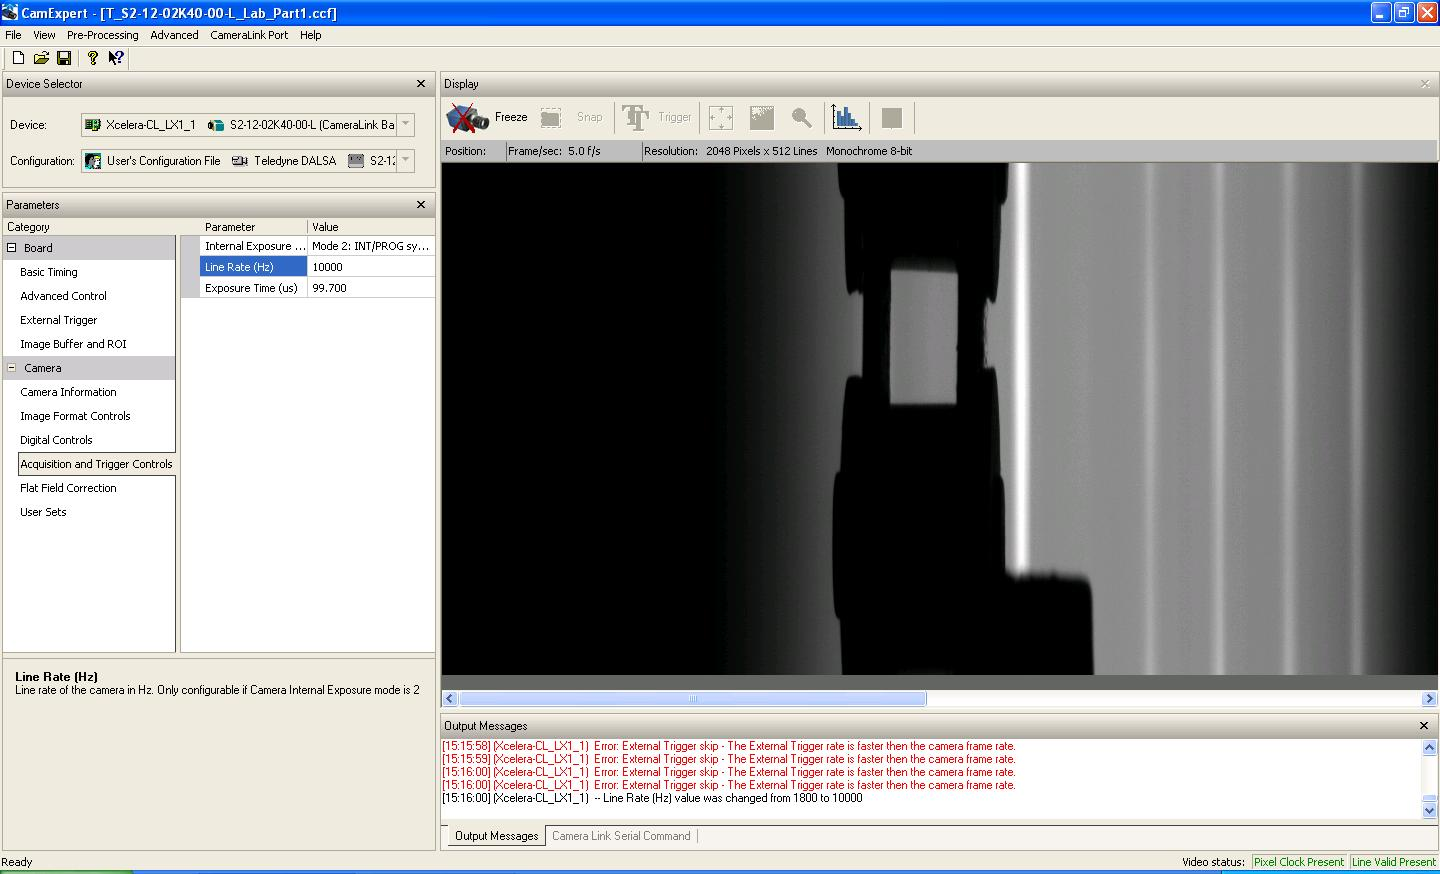
\includegraphics[width=\linewidth]{Pictures/externel_trigger.JPG}
	\caption{External Trigger changes the frame rate of image}
	\label{fig:fourth}
\end{figure}

\section*{Conclusion}
In this experiment we used a line scan camera imaging system and by adjusting some of its settings we discovered its properties. Unlike the classical camera, it only captures one line of an image at a time. Thus, this kind of a camera is intended for imaging when either the camera or the object are moving and the resulting image greatly depends on the speed of the movement.

\section*{References}

{[}1{]} - https://en.wikipedia.org/wiki/Digital\_camera
\\
{[}2{]} - http://www.baslerweb.com/en/products/line-scan-cameras
\end{document}
